\documentclass[11pt]{article}
\usepackage[margin=1in]{geometry}
\usepackage{amsmath,amssymb,amsthm}
\usepackage{graphicx}
\usepackage[hidelinks]{hyperref}

\newtheorem{theorem}{Theorem}

\title{A PSP Subcase of the Property (K) Unconditional-Basis Question}
\author{Literature-implied answer packet for \texttt{fa\_banach\_001}}
\date{\today}

\begin{document}
\maketitle

\section*{Status}

This packet records a \emph{literature-implied partial subcase} of an open
problem from Aviles--Rodriguez \cite{AvilesRodriguez2016}. It is not a full
solution of the problem and not an original proof from this run.

\section*{Source Problem}

Aviles and Rodriguez ask the following as Problem 2.18 of
\cite{AvilesRodriguez2016}:

\begin{quote}
Let \(X\) be a Banach space with unconditional basis not containing subspaces
isomorphic to \(c_0\). Does \(X\) have property (K)?
\end{quote}

The original problem appears together with two other final open questions:

\begin{center}

\includegraphics[width=0.95\linewidth]{figures/open_problem_crop.png}
\end{center}

Here property (K) means that every weak-star null sequence in \(X^*\) admits a
convex block subsequence converging to \(0\) in the Mackey topology
\(\mu(X^*,X)\).

\section*{Supporting Literature}

Rodriguez \cite{Rodriguez2019} introduced the stronger property \((\mu^s)\).
The paper records the implication
\[
(\mu^s) \implies \text{property (K)}.
\]

\begin{center}
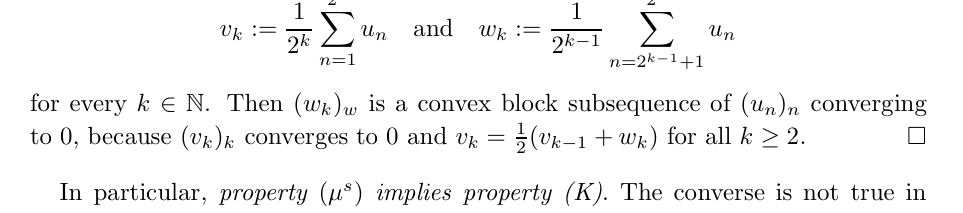
\includegraphics[width=0.95\linewidth]{figures/supporting_mu_to_k_crop.png}
\end{center}

In the Banach-lattice applications, Rodriguez proves that every Banach lattice
with the positive Schur property (PSP) and a weak unit has property \((\mu^s)\):

\begin{center}
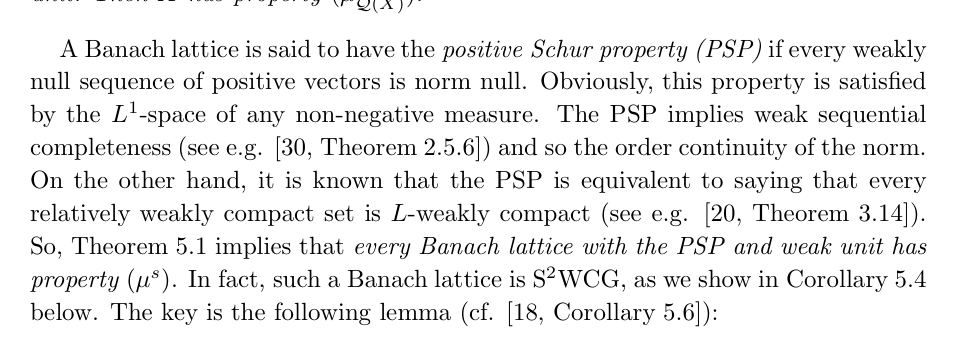
\includegraphics[width=0.95\linewidth]{figures/supporting_psp_mu_crop.png}
\end{center}

\section*{Proof Intuition}

The 2016 problem is difficult because an unconditional basis alone need not
make the Mackey topology on \(X^*\) sequentially manageable. The extra PSP
hypothesis gives a lattice mechanism: in a Banach lattice with PSP, weakly
compact sets are \(L\)-weakly compact, and Rodriguez's theorem turns that
structure into the stronger Mackey-Cesaro property \((\mu^s)\). A countable
unconditional basis supplies a natural coordinate lattice with a weak unit, so
the supporting theorem applies directly to this PSP subfamily.

\section*{Theorem}

\begin{theorem}
Let \(X\) be a Banach space with an unconditional Schauder basis. Equip \(X\)
with the associated coordinate Banach-lattice order. Suppose this Banach
lattice has the positive Schur property. Then \(X\) has property (K).

Consequently, among spaces satisfying the hypotheses of Aviles--Rodriguez
Problem 2.18, the subcase in which the associated unconditional-basis lattice
has the positive Schur property has an affirmative answer.
\end{theorem}

\begin{proof}
Let \((e_n)\) be the unconditional basis. After replacing \(e_n\) by
\(e_n/\|e_n\|\), if necessary, the series
\[
u=\sum_{n=1}^{\infty}2^{-n}|e_n|
\]
converges in \(X\). In the coordinate lattice associated with the
unconditional basis, \(u\) is a weak unit: if \(x\geq 0\) and \(x\wedge u=0\),
then every coordinate of \(x\) is zero, hence \(x=0\).

By the additional hypothesis, this Banach lattice has the positive Schur
property. Rodriguez's Banach-lattice application \cite[Section 5]{Rodriguez2019}
therefore gives property \((\mu^s)\) for \(X\). By \cite[Lemma 2.1 and the
following sentence]{Rodriguez2019}, property \((\mu^s)\) implies property (K).
Thus \(X\) has property (K).

If \(X\) also contains no subspace isomorphic to \(c_0\), then \(X\) lies in
the original class considered in Problem 2.18. The conclusion above is
therefore an affirmative answer for that PSP subcase.
\end{proof}

\section*{Verification Notes}

The supporting paper does not explicitly say that it answers Problem 2.18 of
\cite{AvilesRodriguez2016}. The identification is direct: an unconditional
basis gives a coordinate Banach-lattice structure with a weak unit, and the
supporting PSP theorem gives a property stronger than (K).

The PSP assumption is strictly additional. This packet leaves open the full
question for arbitrary Banach spaces with unconditional basis and no copy of
\(c_0\).

\section*{Bounded Search}

The run indexes were searched for the arXiv ids, property (K), positive Schur
property, PSP, weak unit, unconditional basis, and \(c_0\). Web searches using
exact phrases from the three final open questions in \cite{AvilesRodriguez2016}
found later property (K) papers but no full answer to Problem 2.18. The
supporting result used here is from arXiv:1812.10079.

\begin{thebibliography}{9}

\bibitem{AvilesRodriguez2016}
A. Aviles and J. Rodriguez,
\emph{Convex combinations of weak*-convergent sequences and the Mackey
topology},
Mediterr. J. Math. 13 (2016), 4995--5007.
arXiv:1601.05825.

\bibitem{Rodriguez2019}
J. Rodriguez,
\emph{Cesaro convergent sequences in the Mackey topology},
Mediterr. J. Math. 16 (2019), Paper No. 117.
arXiv:1812.10079.

\end{thebibliography}

\end{document}
